\documentclass[11pt]{article}
 \usepackage[portuguese,brazil]{babel}
 \usepackage{lipsum}
 \usepackage{graphicx}
 \usepackage[colorlinks=true, linkcolor=blue, citecolor=blue, urlcolor=blue]{hyperref}
 \usepackage{eso-pic}
 \usepackage{xcolor}
 \usepackage[round]{natbib} % Adiciona ou ajusta esta linha no preâmbulo para o estilo autor-ano
 \usepackage{indentfirst}
 \usepackage{float}

% Para fonte Arial 
% \usepackage{helvet} % Carrega a fonte Helvetica
%\renewcommand{\familydefault}{\sfdefault} % Muda a fonte padrão para sans-serif (Helvetica)

% Para fonte Times
\usepackage{mathptmx} % Adiciona suporte para a fonte Times
\renewcommand{\familydefault}{\rmdefault} % Garante que a fonte padrão seja serifada




% Definindo a cor azul marinho
\definecolor{navyblue}{RGB}{0,0,128}


\usepackage{analysis_orax}

%------------------Document----------------------------

\begin{document}

%-------------------------TitlePage------------------------
\begin{titlepage}
  \AddToShipoutPictureBG*{%
  \AtPageLowerLeft{%
    
\includegraphics[width=\paperwidth,height=\paperheight]{figures/fundo.png}%
  }%
}

\centering
 % Início do bloco de logos
 \begin{minipage}[b]{0.3\textwidth}
  
\includegraphics[width=\textwidth]{figures/loop.png} % Logo do Loop
\end{minipage}%
\hfill % Espaço entre os logos
\begin{minipage}[b]{0.3\textwidth}
  \centering
  
\includegraphics[width=1\textwidth]{figures/logo.png} % Logo da UFF, ajuste a escala conforme necessário
\end{minipage}%
\hfill % Espaço entre os logos
\begin{minipage}[b]{0.3\textwidth}
  \flushright
  
\includegraphics[width=\textwidth]{figures/petrobras.png} % Logo da Petrobras
\end{minipage}
\\
% Fim do bloco de logos
\vspace{2cm}
{\scshape\Huge \textcolor{navyblue}{Relatório Técnico \# 2} \par} % Aplicando a cor azul marinho
\vspace{1cm}
{\scshape\Large \textcolor{navyblue}{Projeto Ressurgência - Fase IV}\par} % Aplicando a cor azul marinho
\vspace{1.5cm}
{\huge\bfseries \textcolor{navyblue}{Aperfeiçoamento do programa de modelagem de rocha geradoras }\par}
\vspace{2cm}
{\Large\itshape \textcolor{navyblue}{AUTOR: Coloque o seu nome aqui}\par}
\vspace{2cm}
{\Large\itshape \textcolor{navyblue}{COORDENADORES: Ana Luiza S. Albuquerque}\par}
\vfill
{\large \textcolor{navyblue}{\today}\par}




\end{titlepage}

%-------------------------Content------------------------


\section{Isto é uma seção}

\lipsum[5]

    \begin{figure}[H]
    \centering
      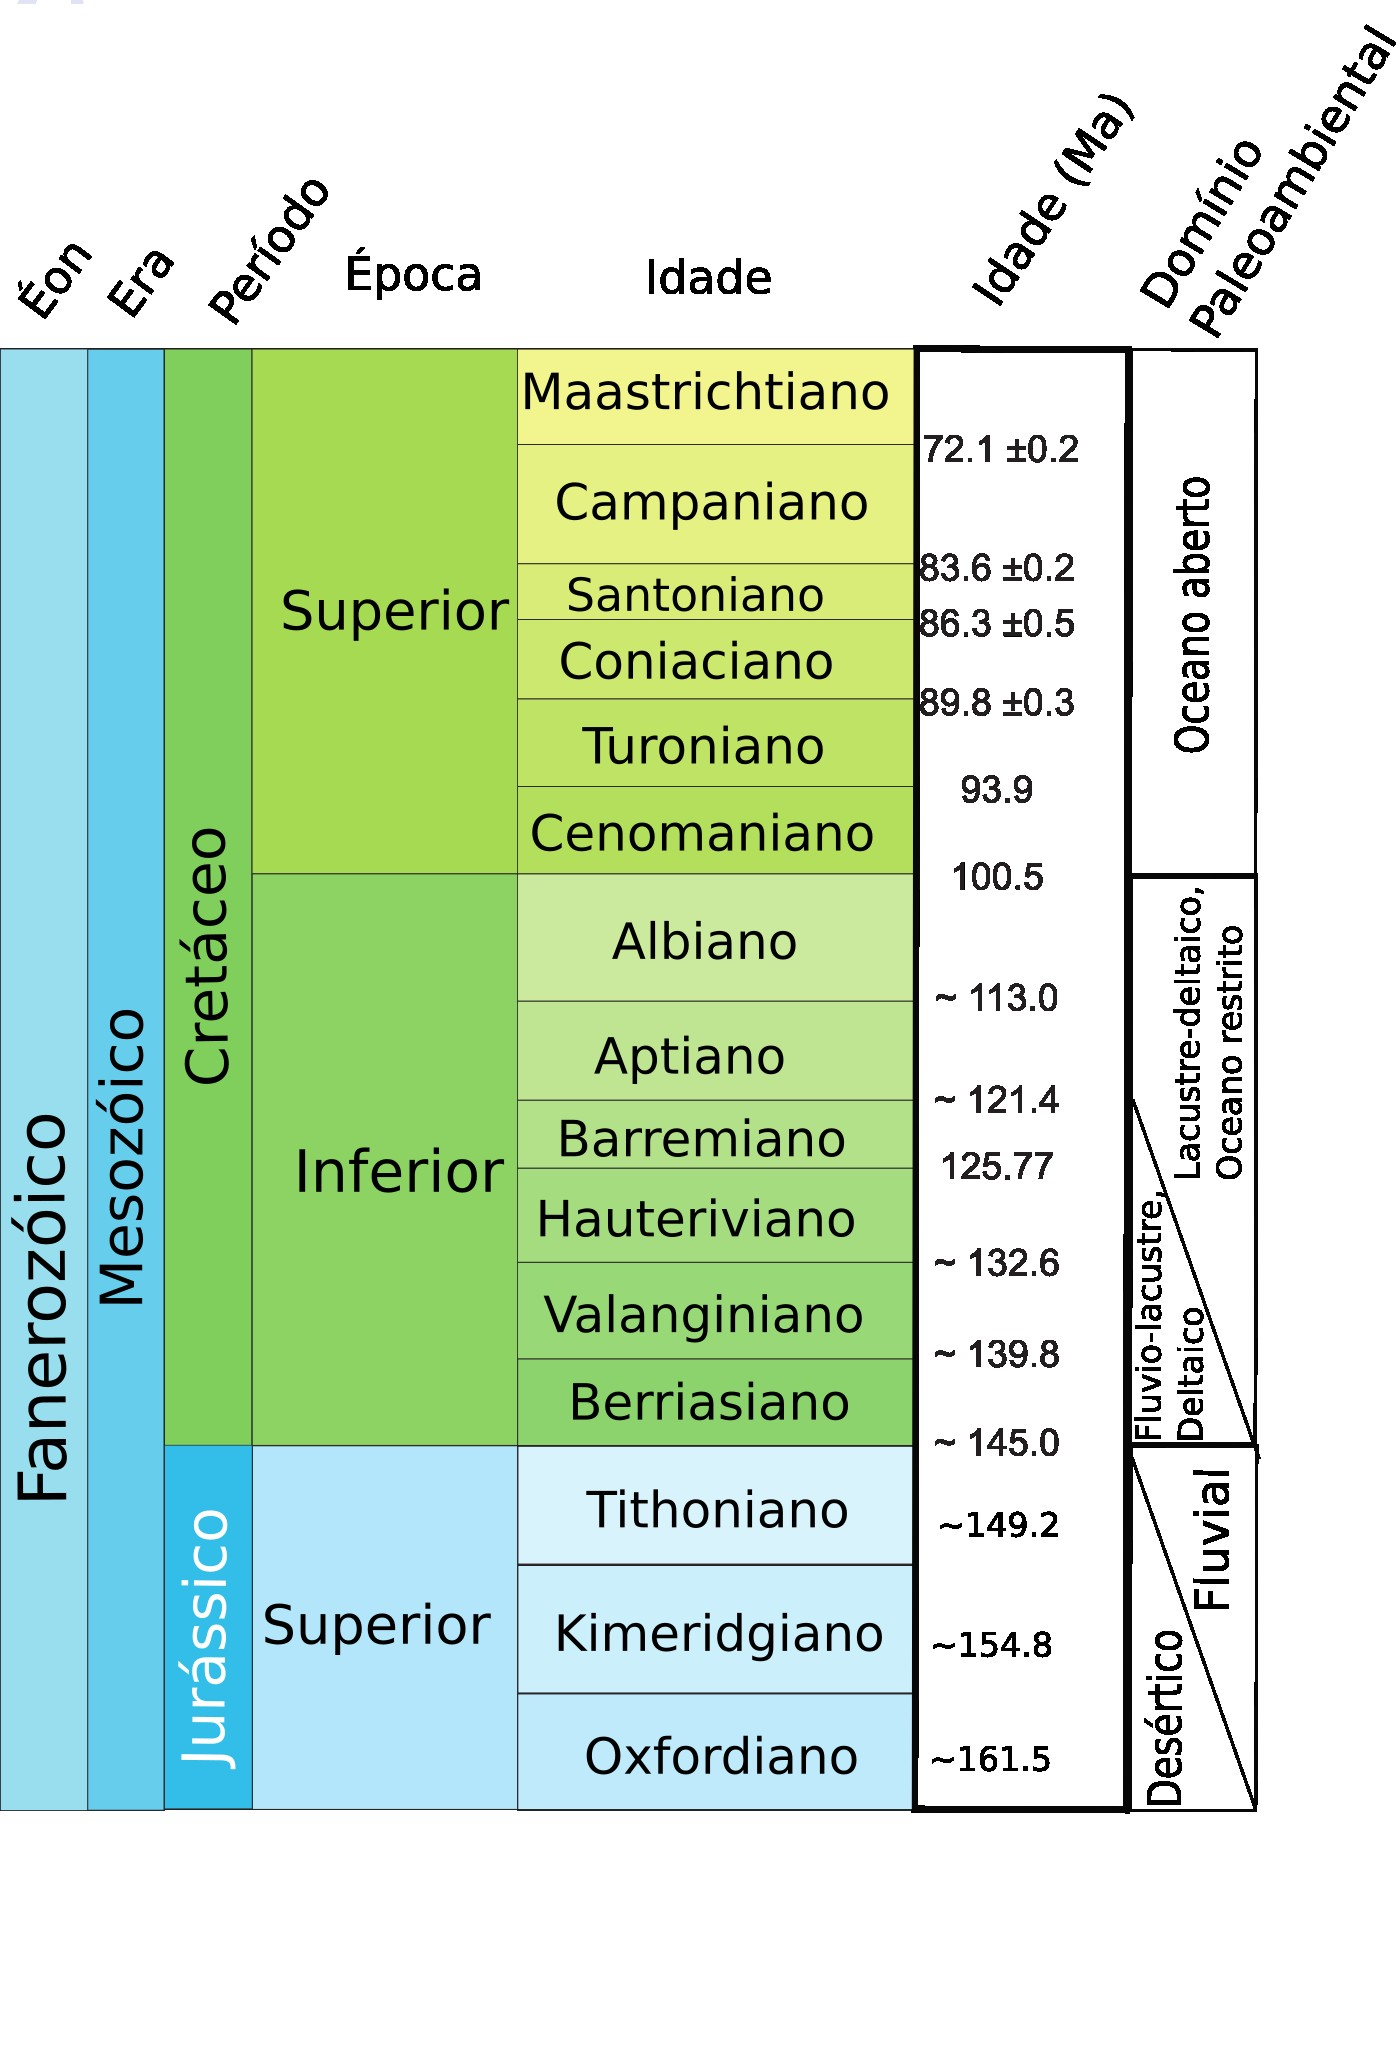
\includegraphics[width=0.5\textwidth]{figures/paleocrono.jpg}
       \centering
	    \caption{\textcolor{Orange}{\textbf{Distribuição dos principais domínios paleogeográficos ao longo do tempo geológico, dentro do contexto evolutivo do rifteamento do atlântico sul. Adaptado da coluna estratigráfica internacional.}}}
	    \label{fig1}
    \end{figure}


\lipsum[5]

\subsection{Isto é uma subseção}
\lipsum[10]

%\newpage
%\section{Desenvolvimento de potenciais produtos}

%\subsection{Proposta de patente do ODISSEU (Kristoffer, Victor)}

\newpage
\bibliographystyle{plainnat} % Ou outro estilo de sua preferência
\bibliography{refs} 

\end{document}
